\documentclass[12pt, titlepage]{article}

\usepackage{fullpage}
\usepackage[round]{natbib}
\usepackage{multirow}
\usepackage{booktabs}
\usepackage{tabularx}
\usepackage{graphicx}
\usepackage{float}
\usepackage{hyperref}


\hypersetup{
    colorlinks,
    citecolor=blue,
    filecolor=black,
    linkcolor=red,
    urlcolor=blue
}

%% Comments
\usepackage{color}
\newif\ifcomments\commentstrue %displays comments
%\newif\ifcomments\commentsfalse %so that comments do not display
\ifcomments
\newcommand{\authornote}[3]{\textcolor{#1}{[#3 ---#2]}}
\newcommand{\todo}[1]{\textcolor{red}{[TODO: #1]}}
\else
\newcommand{\authornote}[3]{}
\newcommand{\todo}[1]{}
\fi
\newcommand{\wss}[1]{\authornote{blue}{SS}{#1}} 
\newcommand{\plt}[1]{\authornote{magenta}{TPLT}{#1}} %For explanation of the template
\newcommand{\an}[1]{\authornote{cyan}{Author}{#1}}
%% Common Parts
\newcommand{\progname}{4TB6 - Mechatronics Capstone} % PUT YOUR PROGRAM NAME HERE
\newcommand{\authname}{Team \#5, Locked \& Loaded
\\ Abi Nevo, nevoa
\\ Elsa Bassi, bassie
\\ Steffi Ralph, ralphs1
\\ Abdul Iqbal, iqbala18
\\ Stephen De Jong, dejons1
\\ Anthony Shenouda, shenoa2} % AUTHOR NAMES                  

\usepackage{hyperref}
    \hypersetup{colorlinks=true, linkcolor=blue, citecolor=blue, filecolor=blue,
                urlcolor=blue, unicode=false}
    \urlstyle{same}


\newcounter{acnum}
\newcommand{\actheacnum}{AC\theacnum}
\newcommand{\acref}[1]{AC\ref{#1}}

\newcounter{ucnum}
\newcommand{\uctheucnum}{UC\theucnum}
\newcommand{\uref}[1]{UC\ref{#1}}

\newcounter{mnum}
\newcommand{\mthemnum}{M\themnum}
\newcommand{\mref}[1]{M\ref{#1}}

\begin{document}

\title{System Design for \progname{}} 
\author{\authname}
\date{\today}

\maketitle

\pagenumbering{roman}

\section{Revision History}

\begin{tabularx}{\textwidth}{p{3cm}p{2cm}X}
\toprule {\bf Date} & {\bf Version} & {\bf Developer}\\
\midrule
January 16, 2023 & 1.0 & Steffi\\
\bottomrule
\end{tabularx}

\newpage

\section{Reference Material}

This section records information for easy reference.

\subsection{Abbreviations and Acronyms}

\renewcommand{\arraystretch}{1.2}
\begin{tabular}{l l} 
  \toprule		
  \textbf{symbol} & \textbf{description}\\
  \midrule 
  \progname & Explanation of program name\\
  \wss{...} & \wss{...}\\
  \bottomrule
\end{tabular}\\

\newpage

\tableofcontents

\newpage

\listoftables

\listoffigures

\newpage

\pagenumbering{arabic}

\section{Introduction}

\wss{Include references to your other documentation}

\section{Purpose}

\wss{Purpose of your design documentation}

\wss{Point to your other design documents}

\section{Scope}

\wss{Include a figure that show the System Context (showing the boundary between
your system and the environment around it.)}

\section{Project Overview}

\subsection{Normal Behaviour}

\subsection{Undesired Event Handling}

\wss{How you will approach undesired events}

\subsection{Component Diagram}

\subsection{Connection Between Requirements and Design} \label{SecConnection}

\wss{The intention of this section is to document decisions that are made
  ``between'' the requirements and the design.  To satisfy some requirements,
  design decisions need to be made.  Rather than make these decisions implicit,
  they are explicitly recorded here.  For instance, if a program has security
  requirements, a specific design decision may be made to satisfy those
  requirements with a password.}

\newpage
\section{System Variables}

%\wss{Include this section for Mechatronics projects}

\subsection{Monitored Variables}

\begin{minipage}{\textwidth}
\renewcommand*{\arraystretch}{1.5}
\begin{tabular}{| p{0.23\textwidth} | p{0.54\textwidth} | p{0.08\textwidth} | p{0.15\textwidth} |}
 \hline
 Variable Name & Description & Type & Units \\ 
 \hline
 m\_SignalEngaged & Monitors whether or not the locking mechanism is engaged & Digital & Boolean \\ 
  \hline
 m\_SignalDisengaged & Monitors whether or not the locking mechanism is disengaged & Digital & Boolean \\ 
  \hline
 m\_SignalClosed& Monitors whether or not the physical mechanism is closed & Digital & Boolean \\ 
  \hline
 m\_Location & Monitors the location of the bike when it is locked & Analog & Coordinates \\ 
  \hline
 m\_BatteryPower & Monitors the current battery percentage & Analog & Percentage \\ 
 \hline
\end{tabular}
\end{minipage}\\

\subsection{Controlled Variables}

\begin{minipage}{\textwidth}
\renewcommand*{\arraystretch}{1.5}
\begin{tabular}{| p{0.25\textwidth} | p{0.52\textwidth} | p{0.08\textwidth} | p{0.15\textwidth} |}
 \hline
 Variable Name & Description & Type & Units \\ 
 \hline
 c\_LockEngaged & Engages the lock & Digital & Boolean \\ 
  \hline
 c\_LocklDisengaged & Disengages the lock & Digital & Boolean \\ 
  \hline
 c\_LockClosed& Indicates to the user that the latch is closed & Digital & Boolean \\ 
  \hline
 c\_BikePosition & Marks the location of the bike when it is locked & Analog & Coordinates \\ 
  \hline
 c\_BatteryPercentStatus & Indicates what the percentage of the battery is & Analog & Percentage \\ 
 \hline
\end{tabular}
\end{minipage}\\

\subsection{Constants Variables - NA}

\newpage
\section{User Interfaces}
There are two user interfaces related to our product. The first is through an application (SmartLock) and the second is the lock itself where the user will be required to manually open/close the chain to secure the bike. \\


The application is where the user will be able to disengage their lock and locate where it was left with the Geotagging feature. \\

 \begin{figure}[h!]
 \begin{center}
 {
  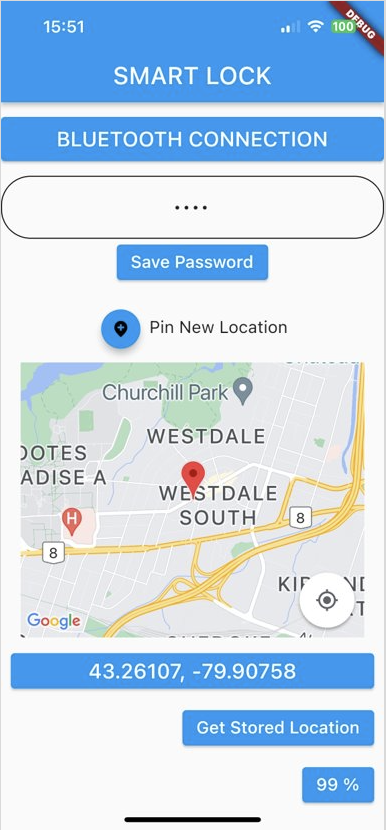
\includegraphics[width=0.5\linewidth]{UI.png}
 }
 \caption{\label{Application User Interface} Application User Interface}
 \end{center}
 \end{figure}

\newpage
The hardware will be mounted to the bike, which will require user interaction upon the purchase of the SmartLock. Additionally, the user must push the locking pin into the hole to engage the lock, and disengage the lock with their phone to be able to remove the pin. 

 \begin{figure}[h!]
 \begin{center}
 {
  \includegraphics[width=0.9\linewidth]{HardwareUI.png}
 }
 \caption{\label{Hardware User Interface} Hardware User Interface}
 \end{center}
 \end{figure}

%\wss{Design of user interface for software and hardware.  Attach an appendix if needed. Drawings, Sketches, Figma}

\section{Design of Hardware}

\wss{Most relevant for mechatronics projects}
\wss{Show what will be acquired}
\wss{Show what will be built, with detail on fabrication and materials}
\wss{Include appendices as appropriate, possibly with sketches, drawings, CAD, etc}

\section{Design of Electrical Components}

\wss{Most relevant for mechatronics projects}
\wss{Show what will be acquired}
\wss{Show what will be built, with detail on fabrication and materials}
\wss{Include appendices as appropriate, possibly with sketches, drawings,
circuit diagrams, etc}

\section{Design of Communication Protocols}

\wss{If appropriate}

\section{Timeline}

\begin{minipage}{\textwidth}
\renewcommand*{\arraystretch}{1.5}
\begin{tabular}{| p{0.12\textwidth} | p{0.38\textwidth} | p{0.50\textwidth} |}
 \hline
 Date & Description & Group Member Assigned\\ 
 \hline
 January 16 & Housing Design & Abi, Elsa \& Steffi\\ 
 \hline
 January 18 & Design Documentation & MG - Elsa \newline MIS - Abi \& Anthony \newline SystDes - Steffi\\ 
  \hline
  January 22 & CAD of Housing Design & Steffi\\ 
  \hline
    January 22 & Circuit & Stephen\\ 
  \hline
    January 22 & App & Anthony\\ 
    \hline
    January 22 & Arduino Coded & Abi\\ 
  \hline
   January 25 & Arduino and Circuit Testing & Abi \& Stephen\\ 
  \hline
   January 29 & Housing 3D Printed & Abdul\\ 
  \hline
    February 1& Assemble Housing and Circuit & Steffi \& Stephen\\ 
  \hline
   February 1& All Documentation has been updated to reflect current project including Git issues \& battery calculations& Elsa\\ 
  \hline
      February 4 & Rev 0 Testing & Everyone\\ 
  \hline
  February 6 & Rev 0 Demonstration & App \& Arduino - Anthony \& Abi \newline Circuit - Stephen \newline Housing - Steffi \& Elsa \newline Documentation Elsa \& Steffi\\
  \hline
  March 8 & V \& V Report Rev 0 & Everyone \newline(Reqs divided by area of expertise on Rev 0 Demonstration)\\
  \hline
 March 20 & Final Demonstration & Everyone \newline(Divided by areas of work)\\
 \hline
 April 5 & Final Documentation & Everyone \newline(Divided by areas of work)\\
 \hline
 TBD & EXPO & Everyone (Divided by areas of work)\\
 \hline
\end{tabular}
\end{minipage}\\




%\wss{Schedule of tasks and who is responsible}

% \bibliographystyle {plainnat}
% \bibliography{../../../refs/References}

\newpage{}
\section{Appendix}

\subsection{Interface - included in section 8}

%\wss{Include additional information related to the appearance of, and interaction with, the user interface}

\subsection{Mechanical Hardware}

\subsection{Electrical Components}

\subsection{Communication Protocols}
%Communication protocols are if you are broadcasting or receiving messages.  If your project doesn't do this, then you don't need to worry about this section.

\subsection{Reflection}

The information in this section will be used to evaluate the team members on the
graduate attribute of Problem Analysis and Design.  Please answer the following questions:

\begin{enumerate}
  \item What are the limitations of your solution?  Put another way, given
  unlimited resources, what could you do to make the project better? (LO\_ProbSolutions)
  \item Give a brief overview of other design solutions you considered.  What
  are the benefits and tradeoffs of those other designs compared with the chosen
  design?  From all the potential options, why did you select documented design?
  (LO\_Explores)
\end{enumerate}

\end{document}